\documentclass[../Main.tex]{subfiles}
\begin{document}

    This chapter describes the background necessary for our work. At the beginning we describe the core concepts of machine learning and image style transfer. Subsequently, the key elements of neural network are briefly outlined.

\subsection{Machine Learning} 
    Machine Learning is the field of study that gives computers the capability to learn without being explicitly programmed. \bartek{add quote: Arthur Samuel}. Technically, machine learning is an approach to data science and analysis that involves adapting and building special models, which allow computer programs to learn through experience. It is based on many others fields such as: linear algebra, calculus, statistics and probability or graph theory. ML models are constructed and improved by algorithms which goal is to make the most accurate possible prediction.
    
    There are various ML concepts and architectures, but one can highlight three most common parts:
    \begin{itemize}
        \item Model - the part which makes predictions
        \item Parameters - the factors used by the model to make decisions
        \item Learner - the part that adjusts the parameters
    \end{itemize}
    Machine Learning works by gathering the data (where quality of data determines the future quality of model), processing to make them consistent and relevant and split them to different sets (usually training and test sets). Next, the chosen algorithm and techniques build the model which is evaluated and upgraded several times to reach the appropriate level of prediction.
    
     One way that we can classify the tasks that machine learning algorithms solve is by how much labeled data they got and how much feedback they present. In some scenarios, the significant amount of labeled data is provided and the model generates some output. This paradigm is called supervised learning. In other cases, no labeled data is provided, no feedback generated - it is an unsupervised learning. Lastly, the reinforcement learning, rather different from the previous ones taking suitable action to maximize reward in a particular situation. The three main paradigms of ML are depicted on Figure \ref{fig:ML-paradigms}.
    
    \begin{figure}[h]
        \centering
        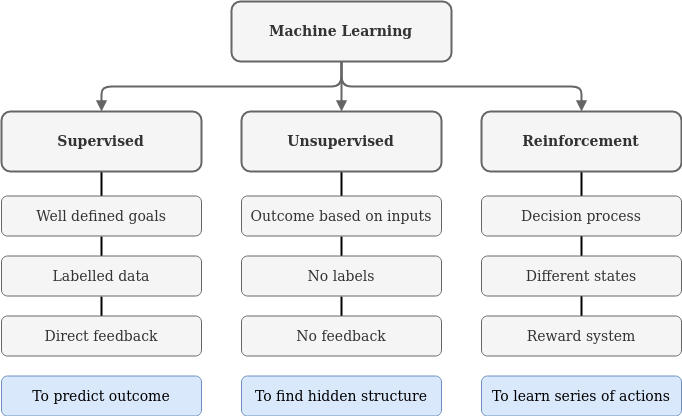
\includegraphics[width=0.7\textwidth]{ML-paradigms}
        \caption{Machine Learning paradigms}
        \label{fig:ML-paradigms}
    \end{figure}

\newpage
    There are whole bunch of different applications to which machine learning methods can be applied. The most popular ones incl.: Natural Language Processing, Classification Problems, Learning Associations, Pattern Recognition and Image Processing which is the one we focus on in this paper.
    \bartek{sources:
    https://deepai.org/machine-learning-glossary-and-terms/machine-learning
    https://martechtoday.com/how-machine-learning-works-150366
    https://developers.google.com/machine-learning/glossary
    }

\subsection{Computer Vision}
    Computer vision is a field of computer science which tries to understand the images and videos - how they are stored, how can we manipulate and effectively retrieve data from them. It seeks to replicate human vision system and enable computers to 'think and see' the same way we do.  Computer Vision plays a major role in photo correction apps and art generation but also in self-driving vehicles or robotics.
    
    Thanks to growing popularity of AI and recent innovations in the field of Deep Learning (and Neural Network as well), Computer Vision develops rapidly and is able to achieve better rates in almost all areas. In many tasks it even can surpass humans (e.g. in object detection and labeling). Since we generate and collect more data used to train and make Computer Vision better, the growth of this field will be ensured.
        \bartek{add source: https://towardsdatascience.com/everything-you-ever-wanted-to-know-about-computer-vision-heres-a-look-why-it-s-so-awesome-e8a58dfb641e
        https://www.bitdegree.org/tutorials/what-is-deep-learning/
        }

\newpage
\subsection{Style transfer}
%  przydałoby się opisać transfer stylu, rozwój prac od 2015
% do 2018, funkcję straty dla transferu stylu, jej interpretację, na czym polega
% AdaIn (https://arxiv.org/abs/1703.06868), czemu była całkeim okej ale nie do końca.
% Takie jej ograniczenia, które ta praca, na której bazujemy rozwiązuje
    \subsubsection{Overview}
    Style transfer is a technique of extraction visual aspects from an image and blending it together with an another image content. It aims to manipulate digital pictures (or videos) and adopt the appearance or visual style. This is usually implemented by optimizing the output image to match the content statistics of the content image and the style statistics of the style reference image. These statistics are extracted from the images using a convolutional network. 
    
    The crucial part of style transfer is process of isolating the style and the content from an image. Researchers developed many approaches which enable computers to do it with high precision. We will go through these techniques in next sections. 
        \bartek{image: https://mspries.github.io/OpticalIllusionReportPage.html
    based on paper: https://arxiv.org/abs/1607.08022
    }
    \\
    \begin{figure}[h]
        \centering
        \includegraphics[width=0.7\textwidth]{style-and-content}
        \caption{Style and content diagram from \href{https://mspries.github.io/OpticalIllusionReportPage.html}{mspires.github.io}}
        \label{fig:style-and-content}
    \end{figure}

    \subsubsection{State of art}
    \bartek[inline]{REWRITE:}
    NST was first published in the paper "A Neural Algorithm of Artistic Style" by Gatys et al., originally released to ArXiv 2015,[2] and subsequently accepted by the peer-reviewed Computer Vision and Pattern Recognition (CVPR) in 2016.[3]
    
    \subsubsection{Loss function}
    
    \subsubsection{AdaIn}
    
    \subsubsection{Examples}
    The most common use of style transfer is obviously the artificial artwork created from photo. Especially the ones produced from some famous paintings. Attached examples give an idea of this approach capabilities. 
    \bartek{attach examples}
    
    image
    
    image
    
    image
    
    \subsubsection{Commercial use}
    Some research projects became a base of mobile applications or programs which can be used by everyone for any purpose:
    \begin{itemize}
        \item \href{https://deepart.io}{DeepArt} - free website where one can turn photo into artistic image
        \item \href{https://www.fritz.ai}{Fritz} - machine learning platform for iOS and Android 
        \item \href{https://prisma-ai.com}{Prisma} - photo-editing application able to create artwork from image
    \end{itemize}
    
    \subsubsection{Alternative approach}
    The alternative CNN approach which used to be popular beforehand is called \textbf{image analogy}. In brief, the algorithm wants to find an analogous image B' that relates to B in the same way as A' relates to A. \bartek{cite: https://mrl.nyu.edu/publications/image-analogies/analogies-72dpi.pdf} To transfer the style of image we need a dataset of training pairs of photo and an artwork from processed photo. The main weakness of this method is that mentioned pair barely exist in practice. An artwork is seldom based on a particular photo.
    
\subsection{Neural Networks}

\bartek[inline]{moge opisac reszte}

    \subsubsection{Overview}
    \subsubsection{Layers}
        \textbf{Fully Connected Layers}
        \textbf{Convolutional Layers}
    \subsubsection{Loss} %for style tranfer
    \subsubsection{Activation}
        \textbf{ReLU}
    \subsubsection{Backpropagation}

\subsection{Neural network compression}
    Latest neural networks usually have between 2 million and 50 million parameters.
    Older architectures are even heavier - full VGG16 model has as much as
    138 million parameters. In consequence models 
    are often too big for deployment on memory bounded mobile and embedded devices.
    Number of parameters strongly correlates with inference time, which in turn
    prevents real-time inference not only on embedded and mobile
    devices but even on middle-class GPUs. Overcoming these limitations 
    is very active area of research.\\
    \textbf{Specialized architectures} such as MobileNet [\cite{mobilenetv1},
    \cite{mobilenetv2}, \cite{mobilenetv3}] and ShuffleNet [\cite{shufflenetv1},
    \cite{shufflenetv2}], replace full convolutions with bottlenecks of lighweight
    pointwise, depthwise and group convolutions in order to reduce number of 
    arithmetic operations and parameters. MobileNetV3 \cite{mobilenetv3} uses
    Neural Architecture Search to optimize the network for mobile phone CPU
    inference, while discussion in \cite{shufflenetv2} shows what aspects should
    be considered, when designing mobile architecture manually. 
    \textbf{Network pruning} aims to reduce already trained model's size by pruning away
    weights with the least impact on network's quality. [\cite{zhu2017prune}] show
    that for some models even up to $87.5$ weights can be removed with only 
    marginally reduced performance. 
    Because networks are initialized randomly, the least
    important parameters are usually spread across whole network. Naive pruning 
    then results in sparse networks. Their storage is significantly reduced, however
    because available linear algebra libraries are optimized for dense structures,
    their inference time doesn't scale as well. To overcome this, more structured
    methods of pruning were developed, among them filter pruning [\cite{li2016pruning},
    \cite{molchanov2016pruning}]
    and channel pruning [\cite{he2017channel}]. 
    Weight's or weights set's importance can be measured by various heuristics. 
    [\cite{li2016pruning}] prune away the filters with the smallest $\ell_1$ norm.
    This approach easily generalizes to $\ell_p$ norm.
    [\cite{polyak2015}] choose to prune away the filters with
    the smallest activation statistics. More direct methods formulate pruning 
    try to preserve performance metrics (e.g. low loss, high accuracy) on training set. 
    [\cite{molchanov2016pruning}] formulate pruning as optimization problem where
    the goal is preserving original training set loss value, that is minimizing
    $|L_{new} - L_{orig}|$. Curiously changing the goal to $L_{new} - L_{orig}$,
    that is letting the loss drop, degrades the resulting network's performance.\\
    Smaller networks can also be trained with aid of larger ones through process called
    \textbf{knowledge distillation} [\cite{hinton2015distilling}]. 
    The key idea is that activations of certain layers
    contain knowledge which is not present in dataset's labels. For example in network 
    trained for classification, the final softmax layer's outputs are usually 
    interpreted as probabilities of respective classes. These probabilities might indicate,
    that for given input x, $C_1$ is the proper class and class $C_2$ is twice as probable 
    as class $C_3$. If the network is well trained, this means x is more similar to
    objects of class $C_2$, rather than $C_3$. By training new small network to match both
    it's softmax outputs with larger trained network's softmax outputs and proper labels,
    we effectively gain additional training data and ease the training.
    Almost every network's inference time can also be increased by \textbf{quantization}.
    In many deep learning frameworks, computation is by default performed on
    32-bit floating point numbers. Such precision is often required during training to 
    ensure gradient's numerical stability. However given that network's weights have
    relatively small magnitude, in many applications it's unnecessary during inference.
    Modern GPUs enable inference in FP16 and INT8 modes. There has also been work 
    on even lower precision inference, performed on CPUs. 
    %TODO: opisać z tej strony: https://software.intel.com/en-us/articles/lower-numerical-precision-deep-learning-inference-and-training; napisać o obecnym stanie bibliotek co
    % do wsparcia dla kwantyzacji
    
        
% ?        
% \subsection{Image and Video Processing}
%     \subsubsection{Basics}
%     \subsubsection{Examples}


\biblio % Needed for referencing to working when compiling individual subfiles - Do not remove
\end{document}
